\chapter{Force Torque Sensor Compensation}
\label{chapter:ft-sensor-correction}

% ADD: Dar introdução ao capítulo
\par In this chapter... (\textbf{dar a outline do capítulo})

\section{Force Torque Sensor Correction}

\par Importance of the force torque sensor in this work... its going to be needed for a lot of functions

\par Ways of interfacing with the force torque sensor, how it works, the ROS services for zero ft sensor, mention UR configuration parameters payload anf cog

\subsection{Noise Filtering}

\par signal is very noisy

\[ W_{fil} = (1-\alpha)W_n + \alpha \left(\frac{W_n + W_{n-1})}{2}\right) \]

\par good results with alpha = 0.1

\begin{figure}[h]
    \centering
    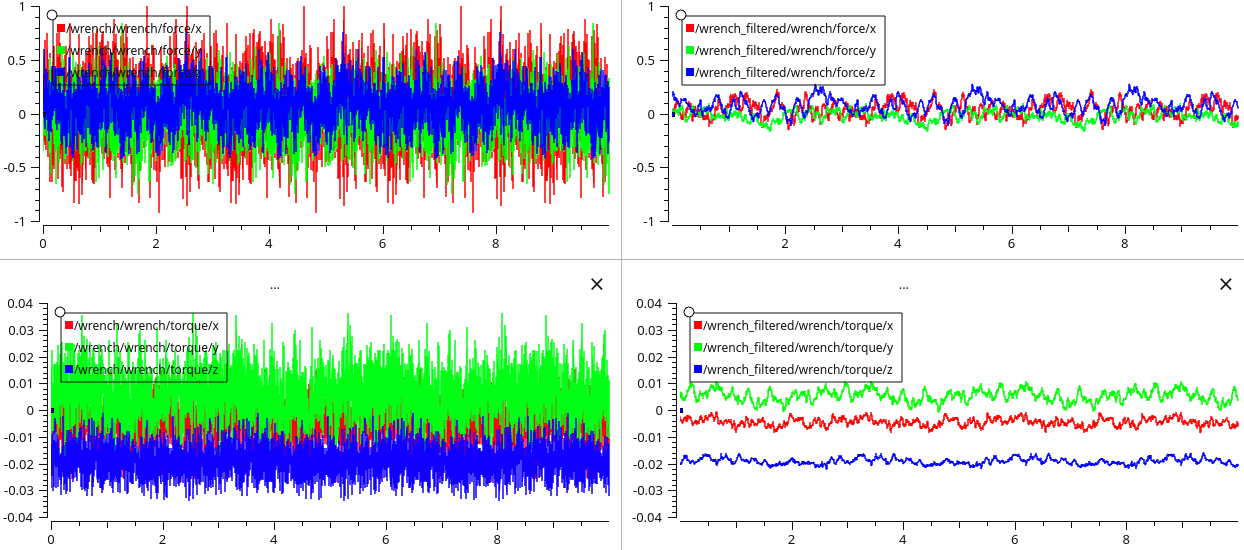
\includegraphics[width=0.9\linewidth]{figs/chp3/ft_sensor_filter.png}
    \caption{Demonstration of the filter node on the wrench values}
    \label{fig:ft_sensor_filter}
\end{figure}

\par Show graph of noise filtered

\subsection{Force Torque Sensor Observed Behavior}

\subsubsection{Wrist 3 Joint Positional Variation}

\par In any pose, the UR10e EEF, in different positions it presents variation in the values of force and torque

\begin{figure}[h]
    \centering
    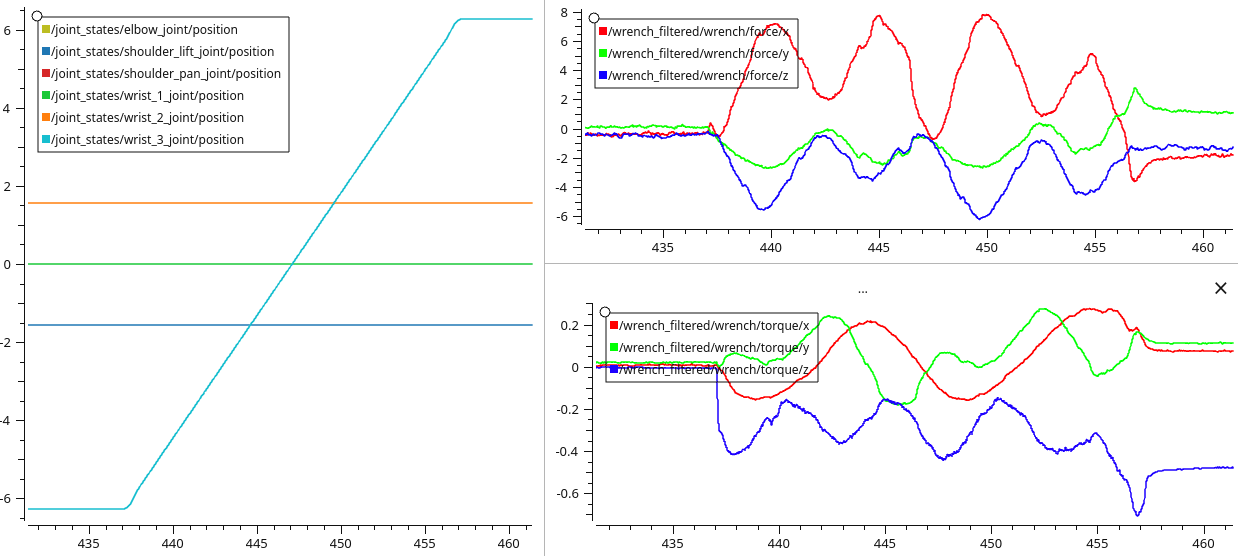
\includegraphics[width=0.9\linewidth]{figs/chp3/wrist_3_problem.png}
    \caption{Wrist 3 Joint Positional Variation}
    \label{fig:w3_problem}
\end{figure}


\subsubsection{Temporal Drift}

\par While the EEF is standing still, variations on the values of FT are presented and increase linearly with time

\begin{figure}[h]
    \centering
    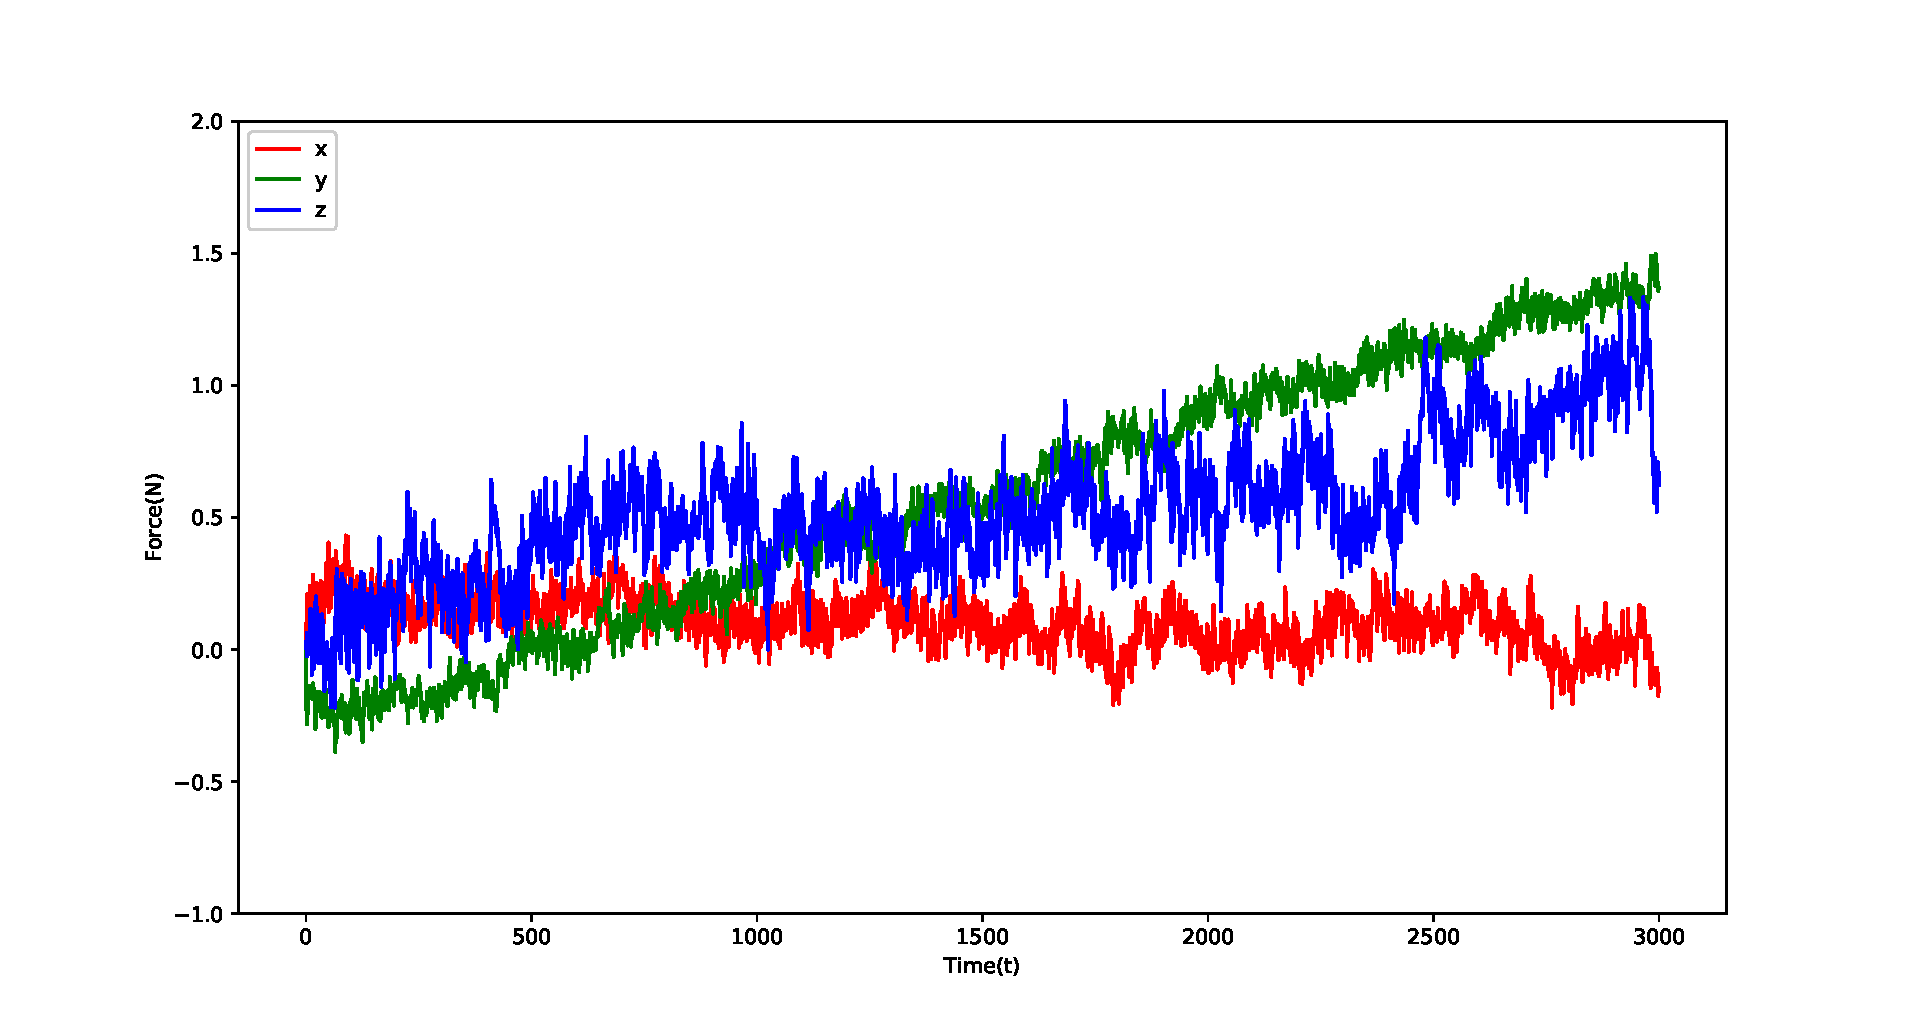
\includegraphics[width=\linewidth]{figs/chp3/ft_sensor_drift.pdf}
    \caption{\ac{ft} Sensor Temporal Drift}
    \label{fig:ft_sensor_drift}
\end{figure}


\subsubsection{Variations caused by \ac{ft} applied}

\par By applying force and torque in the sensor, without the EEF ever changing its position, the values will present variations

\begin{figure}[h]
    \centering
    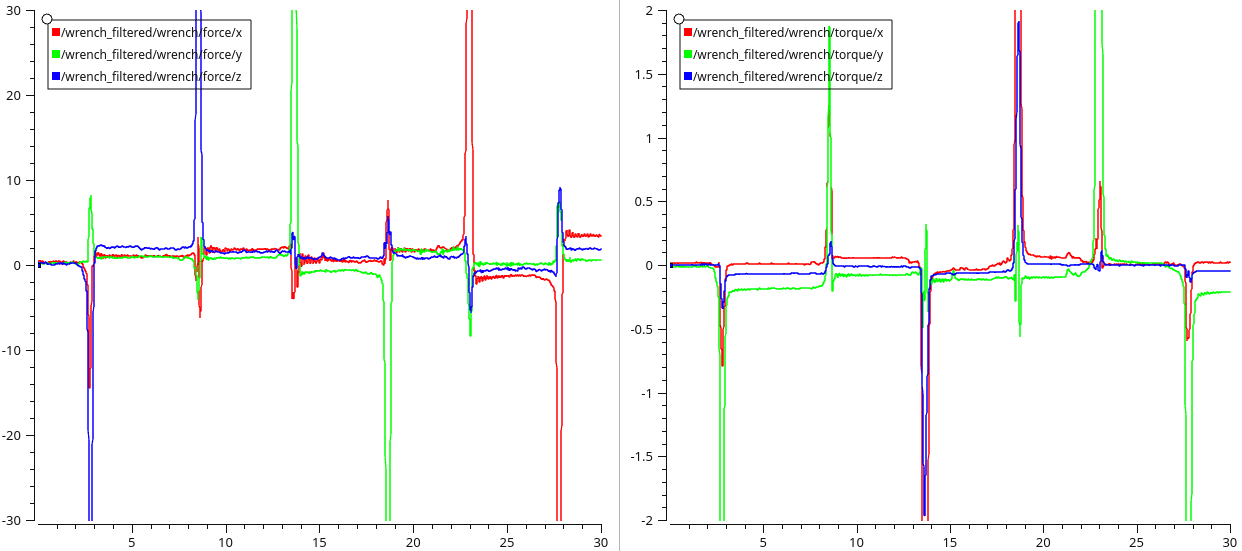
\includegraphics[width=0.9\linewidth]{figs/chp3/ft_sensor_pushes.png}
    \caption{Variation in \ac{ft} affected by pushes in the \ac{eef}}
    \label{fig:ft_sensor_pushes}
\end{figure}

\subsubsection{Special case of the Z-Axis}

\par Values of Z force will present variations depending on the force that the gripper is coupled to the EEF

\par Values of Z torque will present variations when movements in the wrist 3 joint are performed

\subsection{Proposed Solution}

\par Recording values of FT in multiple EEF poses and making variate wrist 3 joint angle from -360 to 360

\begin{figure}[h]
    \centering
    \begin{subfigure}{.195\linewidth}
      \centering
      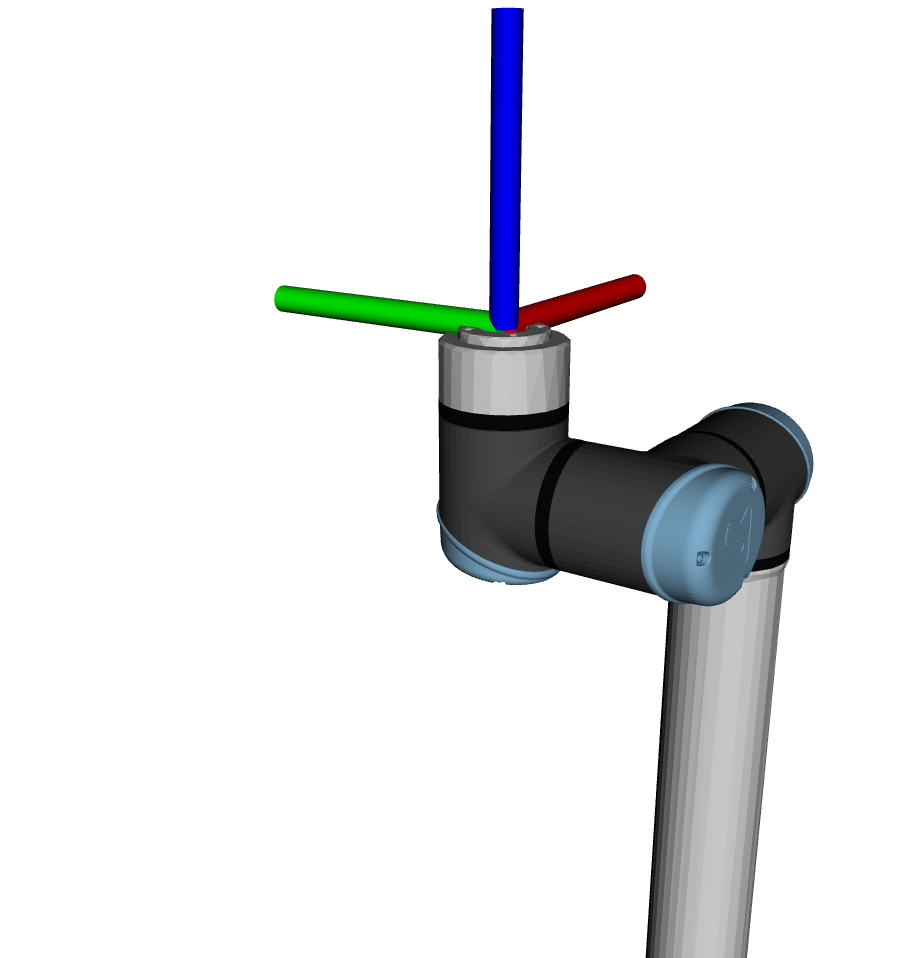
\includegraphics[width=\linewidth]{figs/chp3/P1.png}
      \label{fig:eef_p1}
    \end{subfigure}%
    \begin{subfigure}{.195\linewidth}
      \centering
      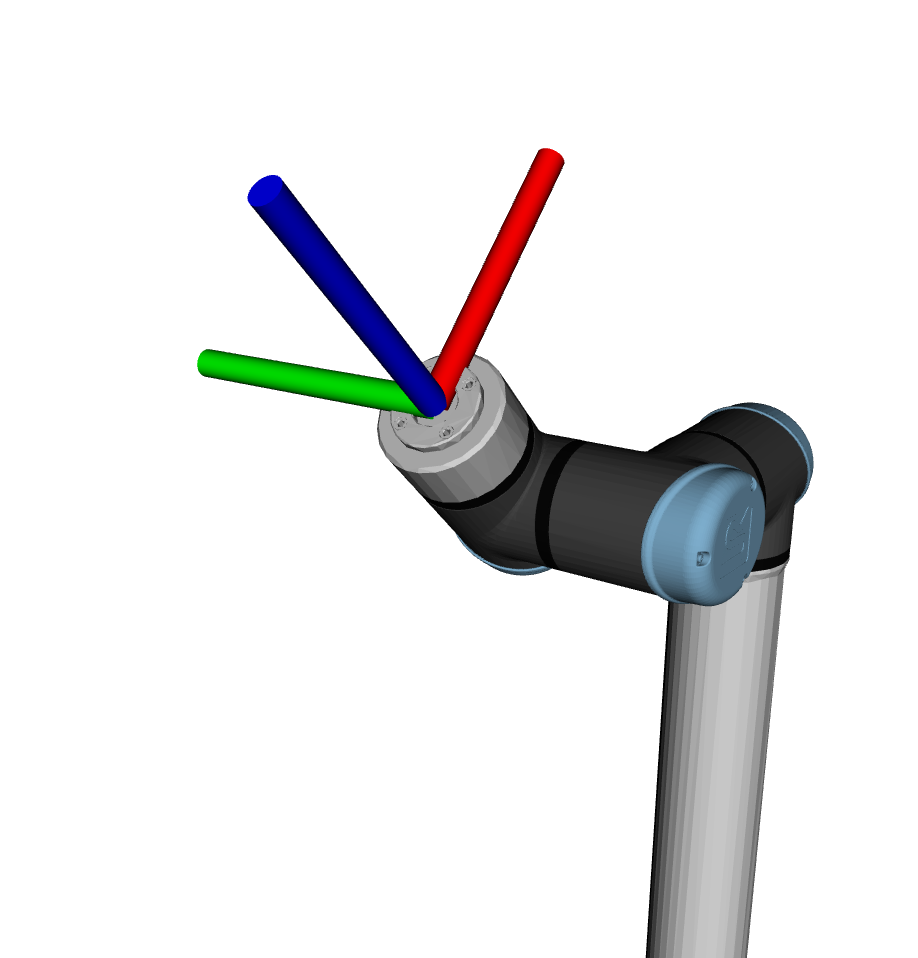
\includegraphics[width=\linewidth]{figs/chp3/P2.png}
      \label{fig:eef_p2}
    \end{subfigure}
    \begin{subfigure}{.195\linewidth}
        \centering
        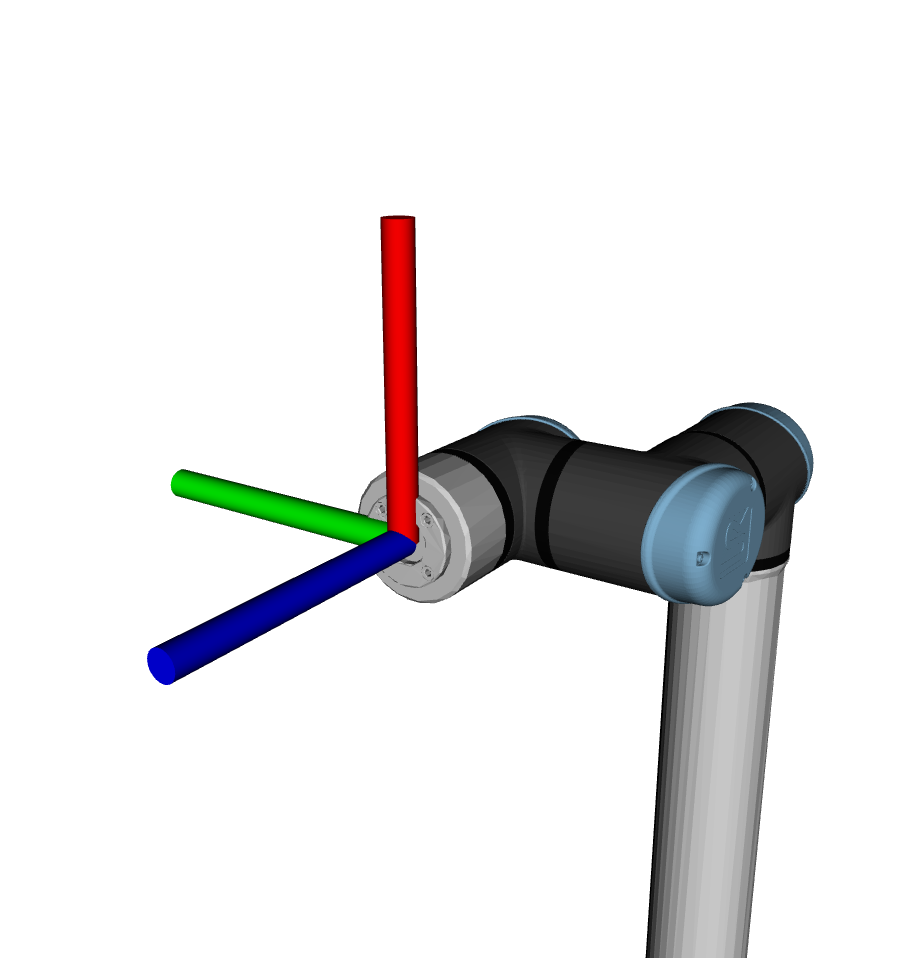
\includegraphics[width=\linewidth]{figs/chp3/P3.png}
        \label{fig:eef_p3}
    \end{subfigure}
    \begin{subfigure}{.195\linewidth}
        \centering
        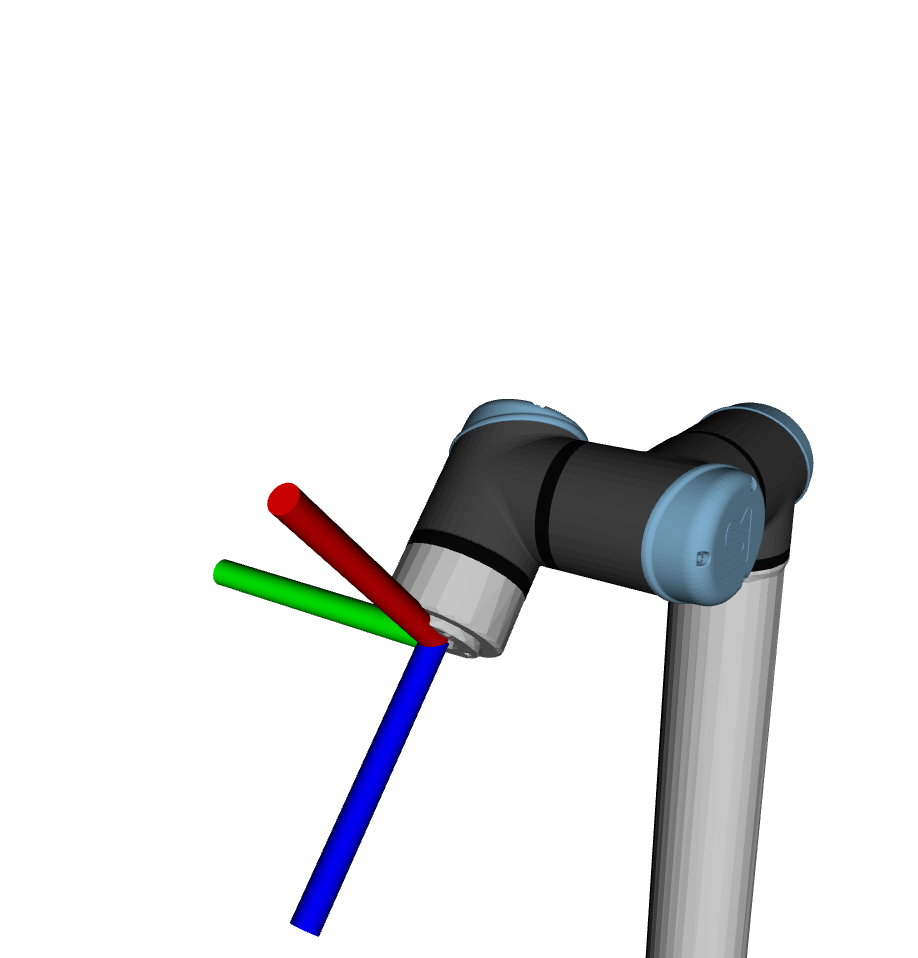
\includegraphics[width=\linewidth]{figs/chp3/P4.png}
        \label{fig:eef_p4}
    \end{subfigure}
    \begin{subfigure}{.195\linewidth}
        \centering
        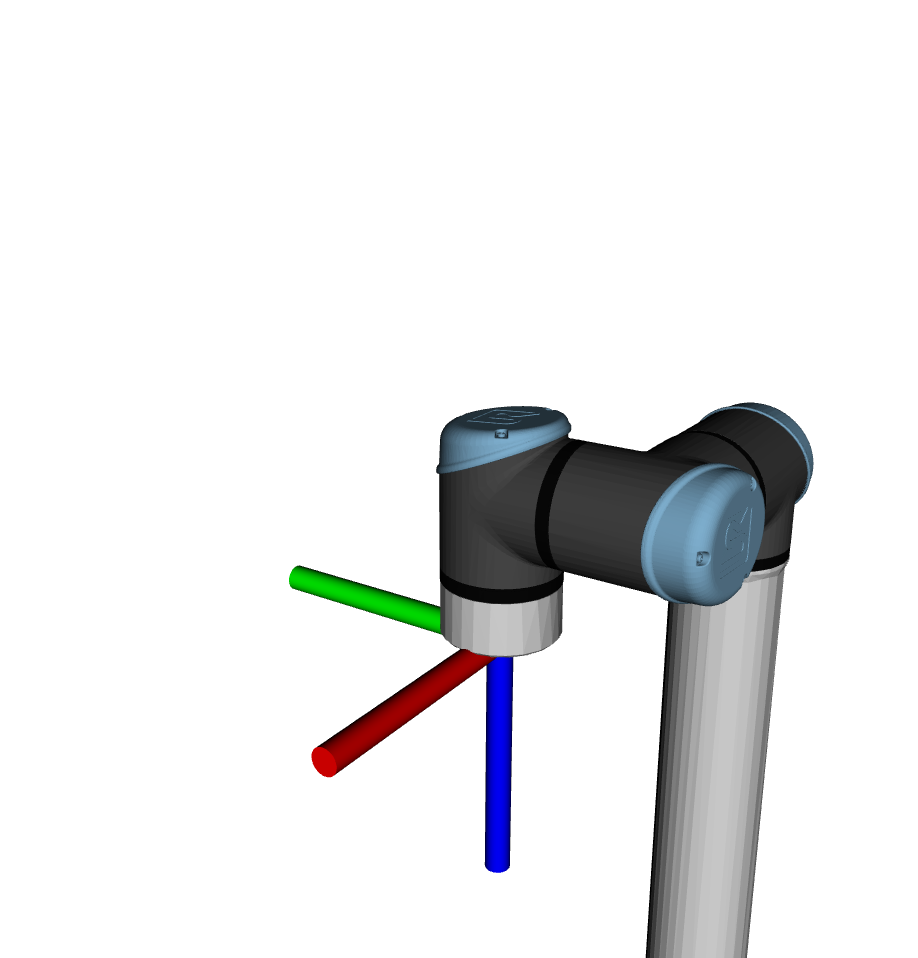
\includegraphics[width=\linewidth]{figs/chp3/P5.png}
        \label{fig:eef_p5}
    \end{subfigure}
    \caption{5 different poses for the \ac{eef}}
    \label{fig:eef_5_position}
\end{figure}

\par In each of these 5 poses a test was made recording the FT values on each angle of the joint wrist 3

\begin{figure}[h]
    \centering
    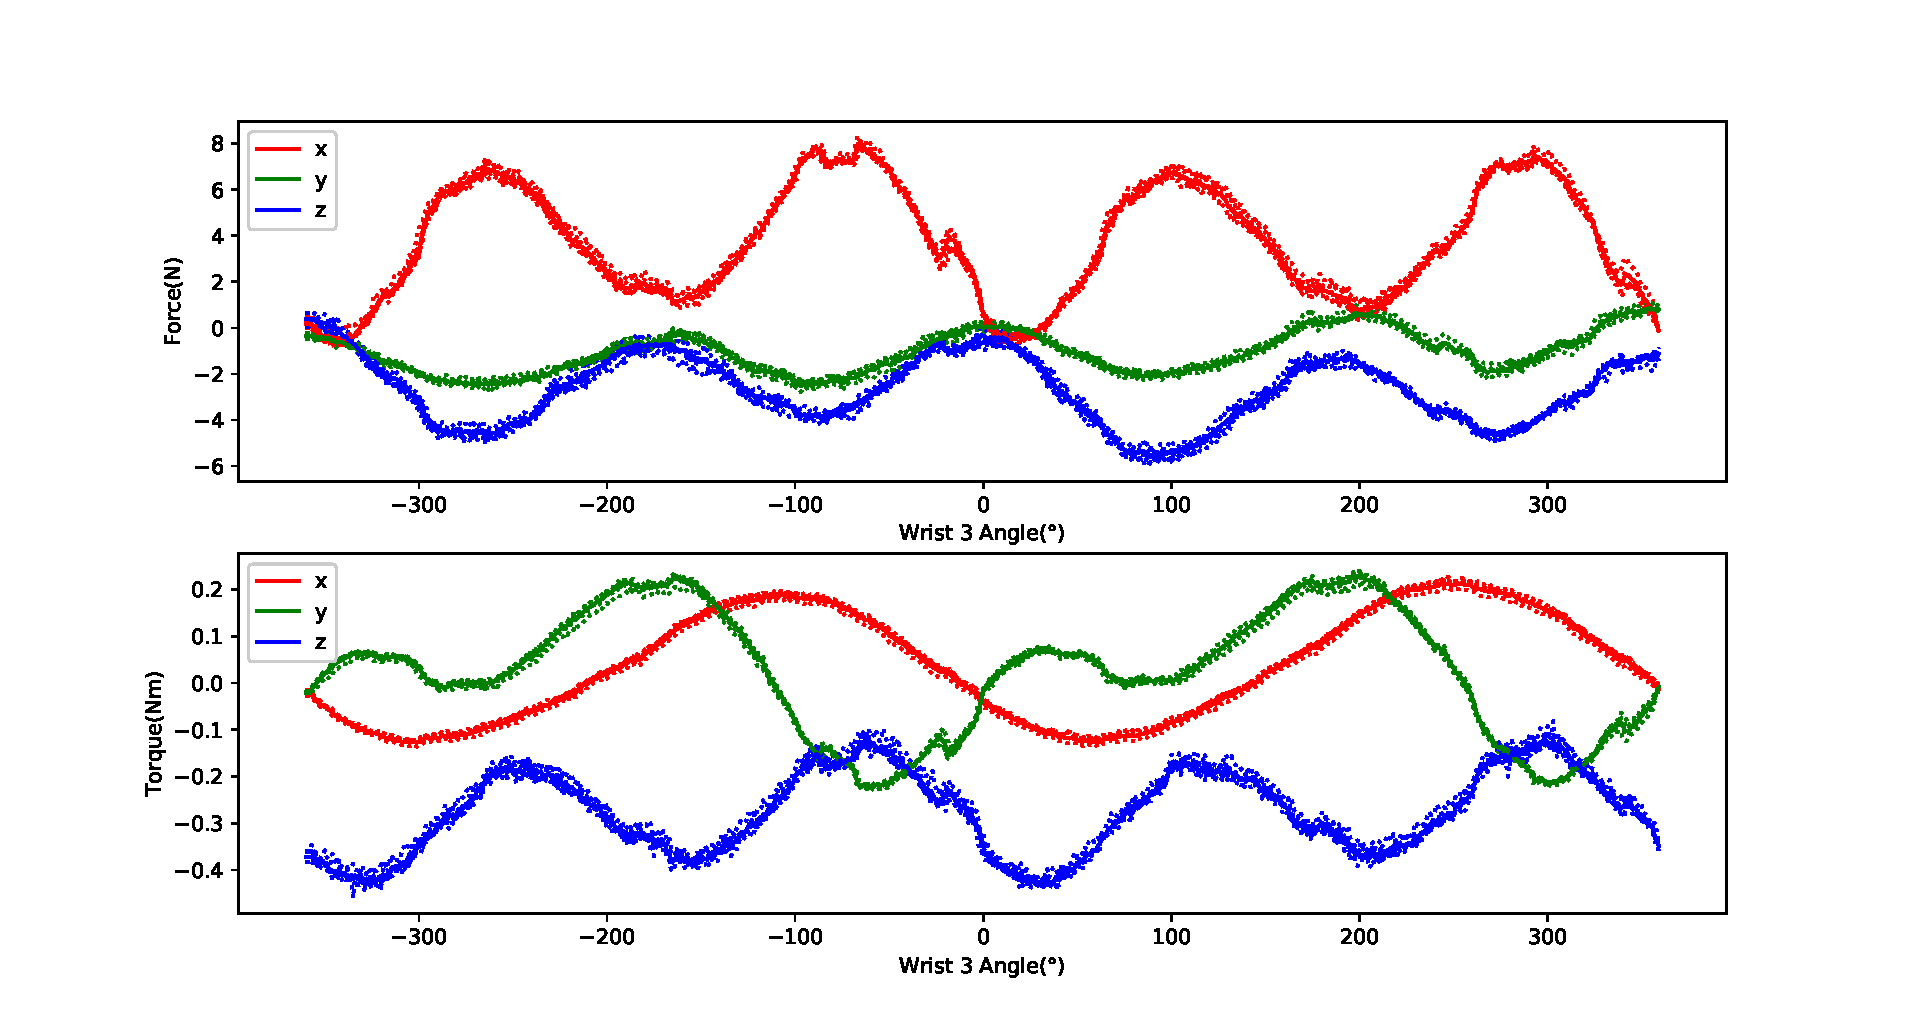
\includegraphics[width=\linewidth]{figs/chp3/ft_sensor_test_5.pdf}
    \caption{Average \ac{ft} values in the 5 defined poses}
    \label{fig:ft_sensor_test_5}
\end{figure}


\par the average of this values will be saved locally and a node will be created that listens to the positions of the w3 and corrects the values coming from wrench in real-time


\par For the remaining problems (drift and shifts when pushes) a separate node will be listening to force changes in real time, when it detects that the user is not interacting with the robot, it will zero the ft sensor, making the pushes and drift problem irrelevant


\subsection{Result}

\par A node was created that listens to the values of ft sensor as corrects them in real-time

\begin{figure}[h]
    \centering
    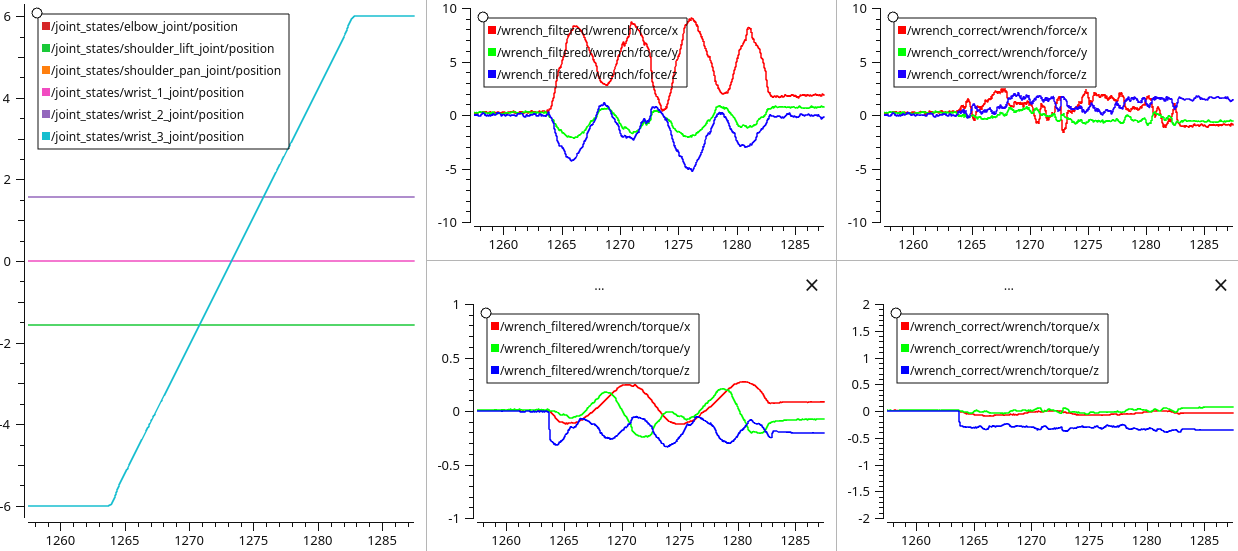
\includegraphics[width=0.9\linewidth]{figs/chp3/wrist_3_result.png}
    \caption{Result of the correction node applied in the initial test}
    \label{fig:w3_result}
\end{figure}

\par Mention that the results are good , that the variation comes from the continuous movement of wrist 3 and that the real difference can be seen on the histogram


\begin{figure}[h]
    \centering
    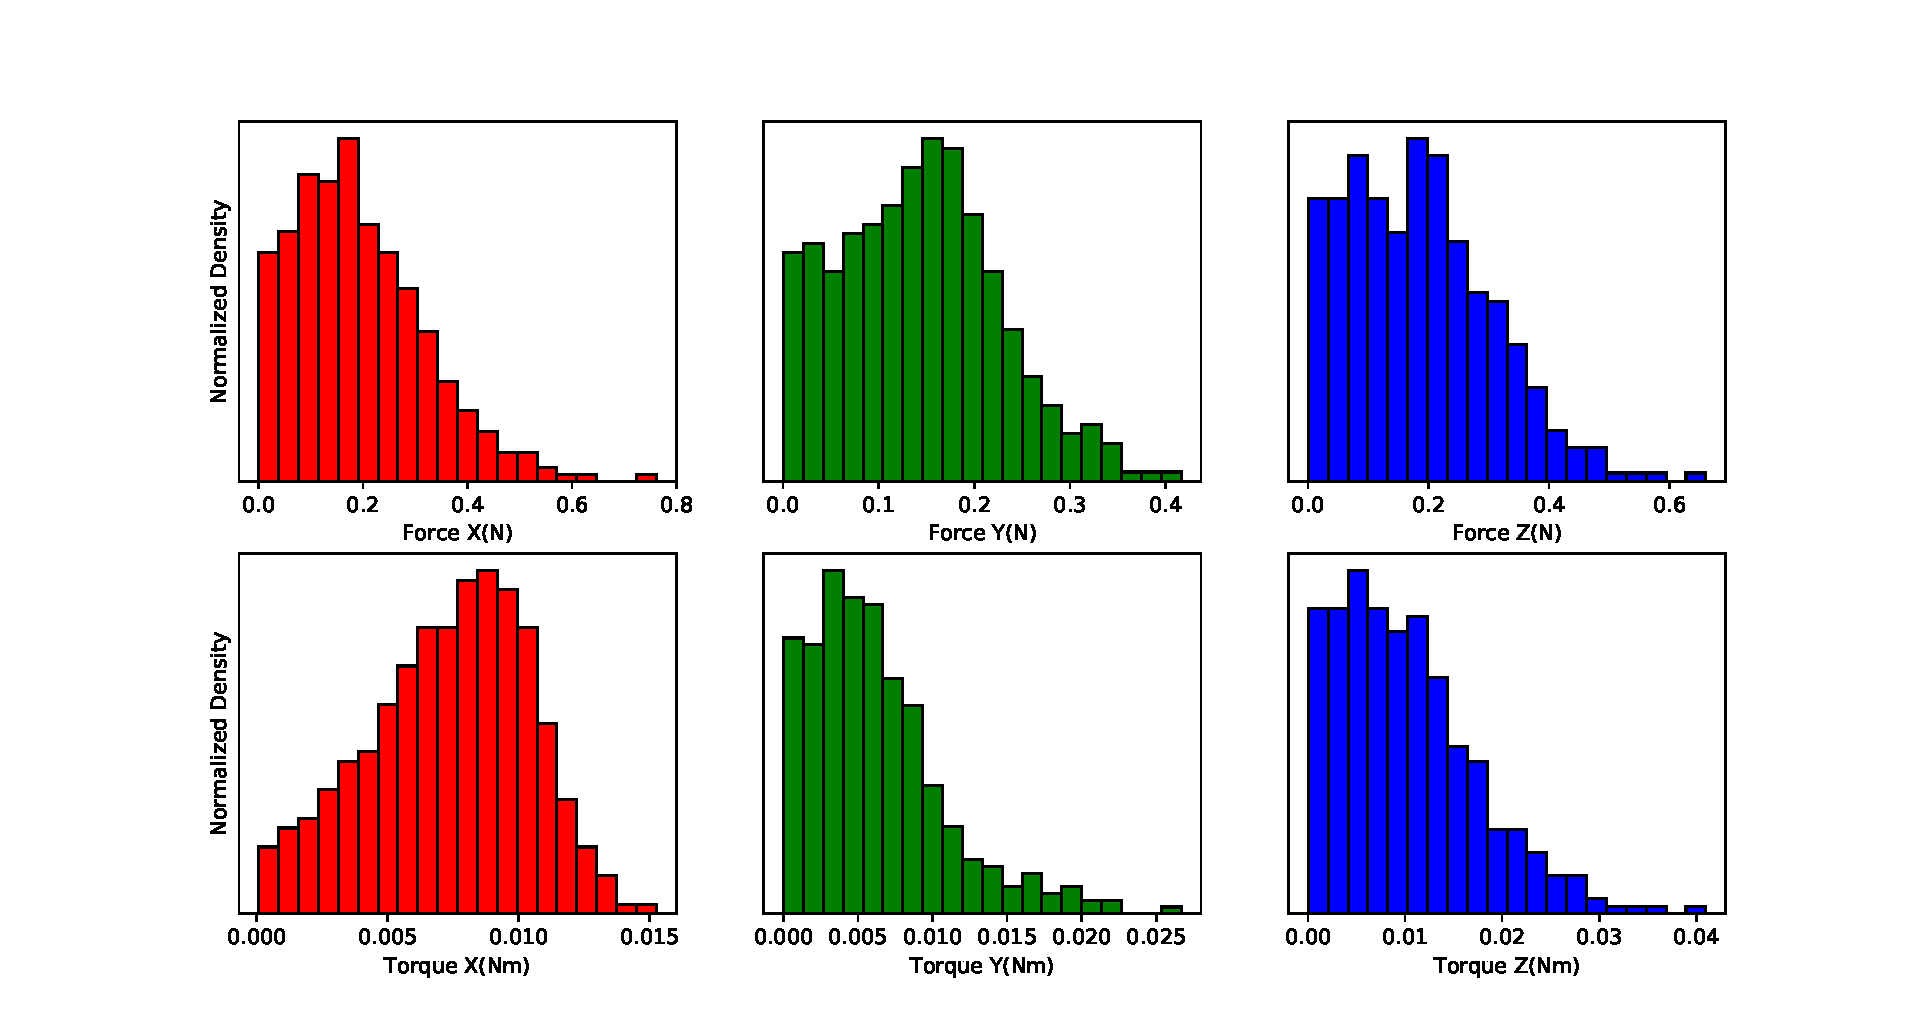
\includegraphics[width=\linewidth]{figs/chp3/wrist_3_result_hist.pdf}
    \caption{Histogram showing the difference from the correct function}
    \label{fig:w3_result_hist}
\end{figure}


\section{End Effector Weight Compensation}

\par For effective hand guide the robot with attached tools and objects, the effects of the weight and cog of the object must be compensated, so a model of the behavior of the FT sensor must be created...

\subsection{UR FT Sensor Controller Internal Compensation}

\par The user only has access to the FT values from that are published by the controller. Furthermore if the user changes the internal payload weight and center of gravity parameters, the controller behavior will change

\par Behavior of the sensor with Payload configured to 1.5Kg and Cog [0, 0, 100] and nothing attached to the EEF

\begin{figure}[h]
    \centering
    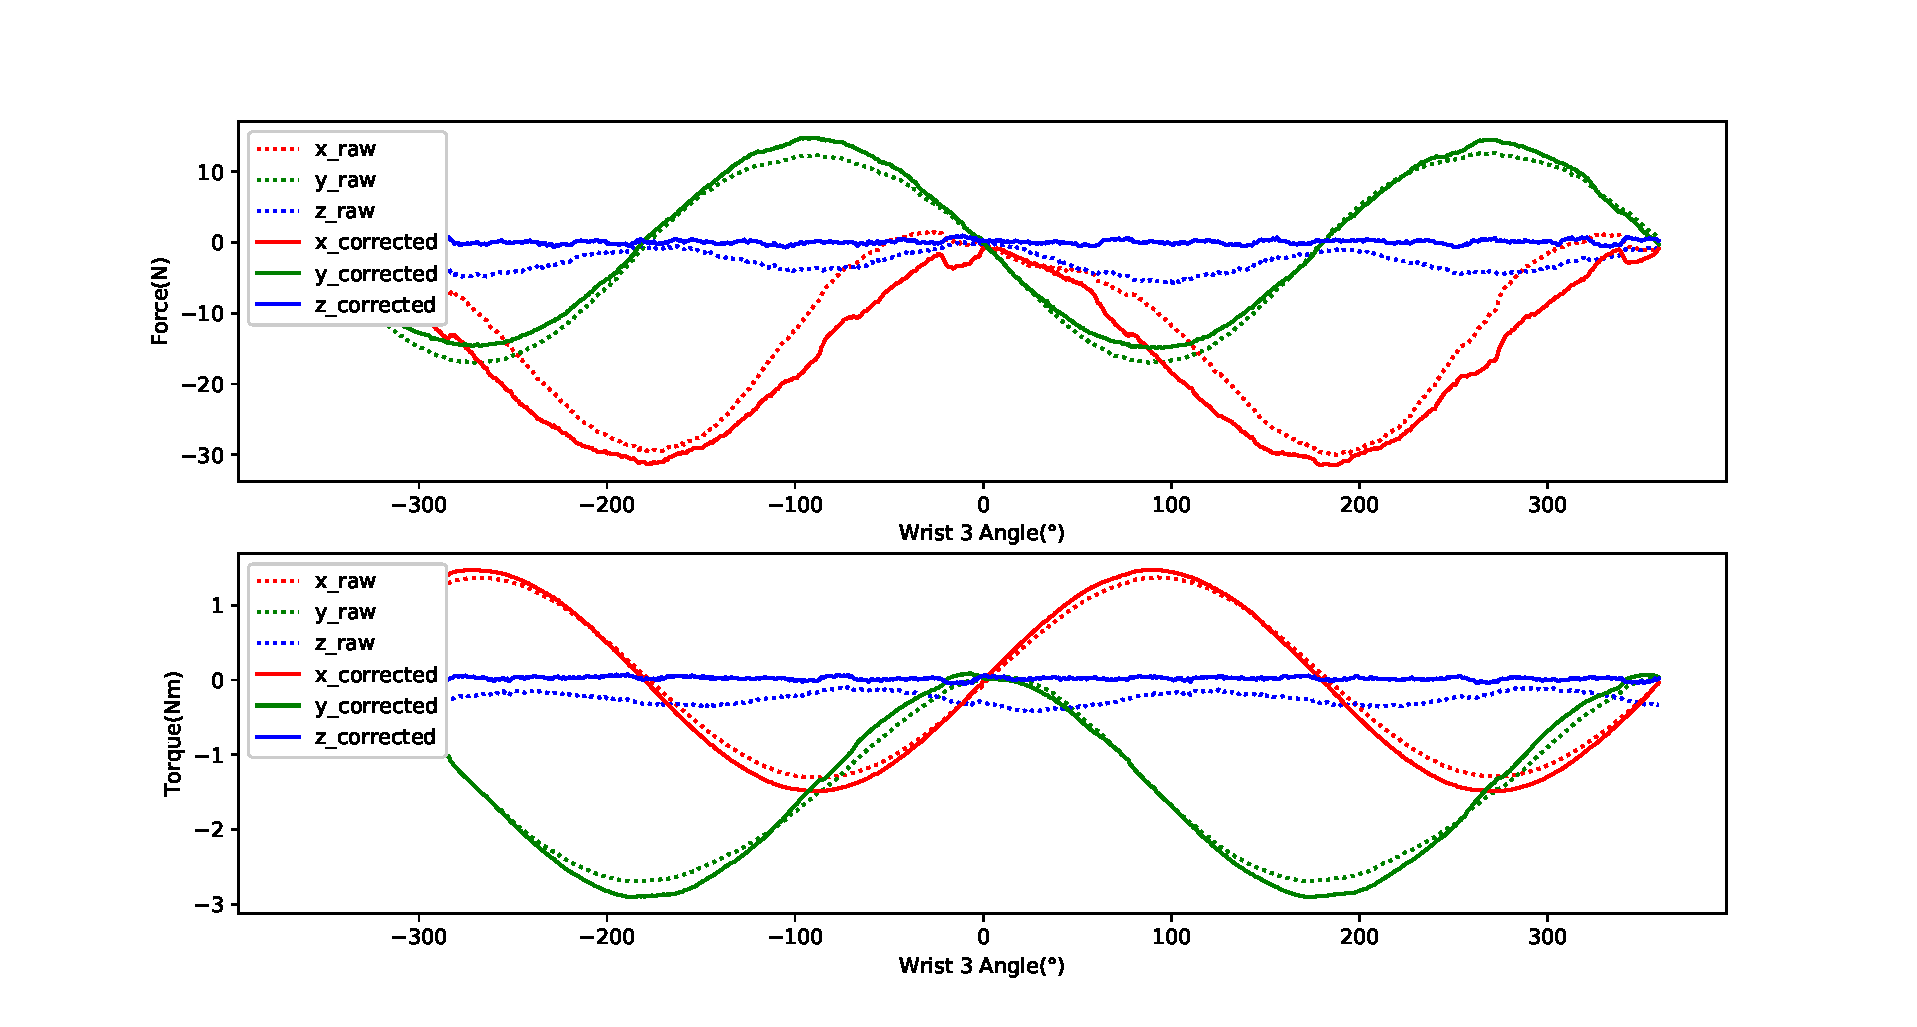
\includegraphics[width=\linewidth]{figs/chp3/ft_sensor_behavior.pdf}
    \caption{Behavior of the FT sensor with parametrization of payload and cog }
    \label{fig:ft_sensor_behavior}
\end{figure}

\par This means that the behavior of the ft sensor changes depending on the configured payload and cog and because there is no knowledge on the implementation of hte controller, the values that will be considered from here forward are payload 0 and cog 0 to get a consistent behavior independent of the weight of hte object 


\subsection{FT Theoretical Model}

\par Based on the knowledge of the weight and cog of the attached object this model should give the theoretical values that a FT sensor should have

\subsubsection{Force}

\par Explain the force generation model

\begin{figure}[h]
    \centering
    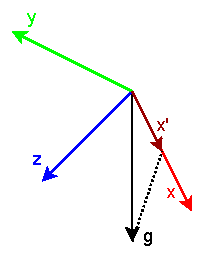
\includegraphics[width=0.3\linewidth]{figs/chp3/ft_theory_force.pdf}
    \caption{Visualization of generation of theoretical force values}
    \label{fig:ft_theory_force}
\end{figure}

\[ Fx = \langle \hat{x_{eef}} , \hat{g} \rangle \cdot m \cdot g \]

\subsubsection{Torque}

\par Explain the torque generation model

\begin{figure}[h]
    \centering
    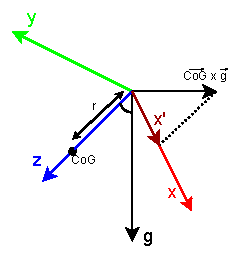
\includegraphics[width=0.35\linewidth]{figs/chp3/ft_theory_torque.pdf}
    \caption{Visualization of generation of theoretical torque values}
    \label{fig:ft_theory_torque}
\end{figure}

\[ Tx = \langle\hat{x_{eef}} , \vec{CoG} \times \vec{g} \rangle \cdot m \cdot g\cdot r \]

% O melhoramento desta função tem a haver com a seguinte divisao
% para a obtenção de um torque em X, ha 3 componentes
%     1 - mg -> sempre
%     2 - que tem a haver com a rotação em Y -> r.sin(theta)
%     3 - que tem a haver com a rotação em Z -> < X , cog x g>
% Tabem pode ser possivel alterar esta equacao para
%     1 - mg -> sempre
%     2 - que tem a haver com a rotacao em Y -> r(vetor com 3 comp) x sin(angulo que faz com o eixo)
%     3 - que tem a haver com a rotação em Z -> projecção do vetor g no plano cujo vetor normal é o eixo

\subsubsection{Results}

\par With a configured weight of 1.5Kg, Cog (0, 0, 0.45) and with an EEF orientation of (specify orientation)

\par below is a comparison of the values from the sensor (corrected) and the theory model

\begin{figure}[h]
    \centering
    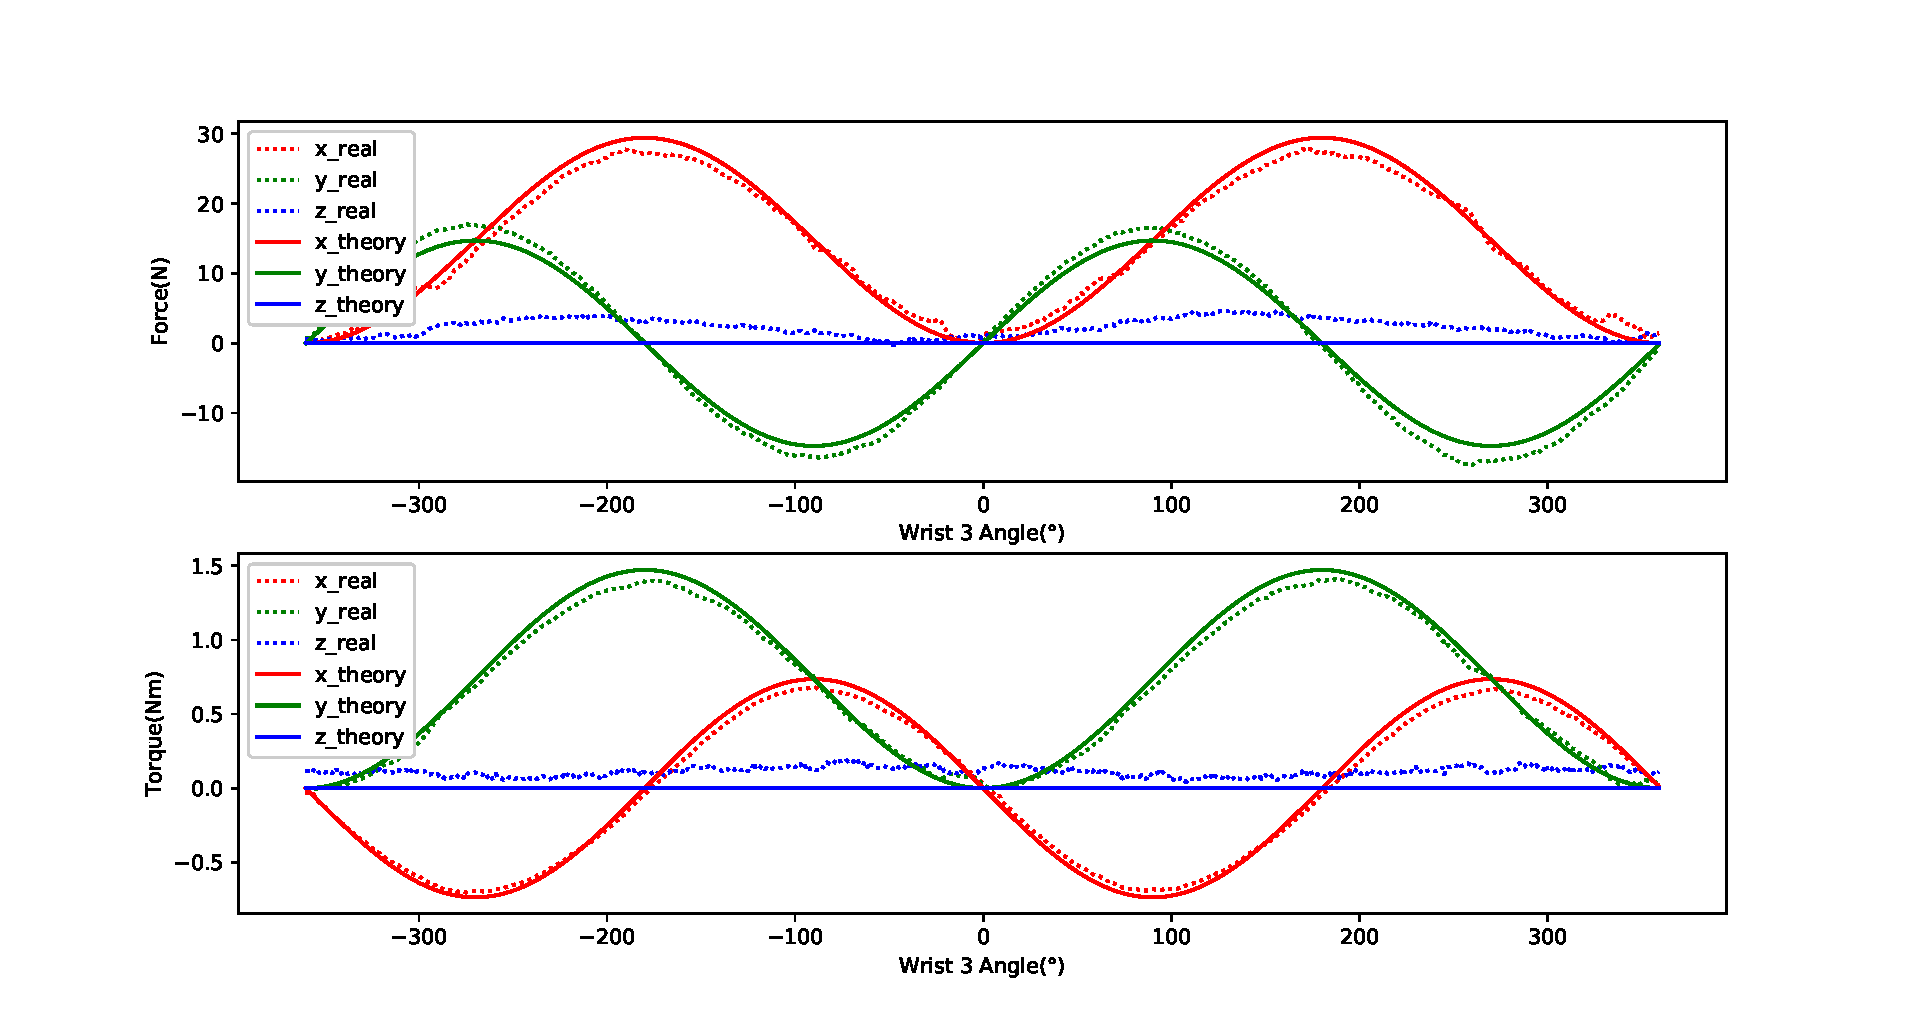
\includegraphics[width=\linewidth]{figs/chp3/ft_sensor_theory.pdf}
    \caption{Visualization of generation of theoretical torque values}
    \label{fig:ft_sensor_theory}
\end{figure}


\par Below is an histogram for a better understanding of the distribution of the erros between the 2 things

\begin{figure}[h]
    \centering
    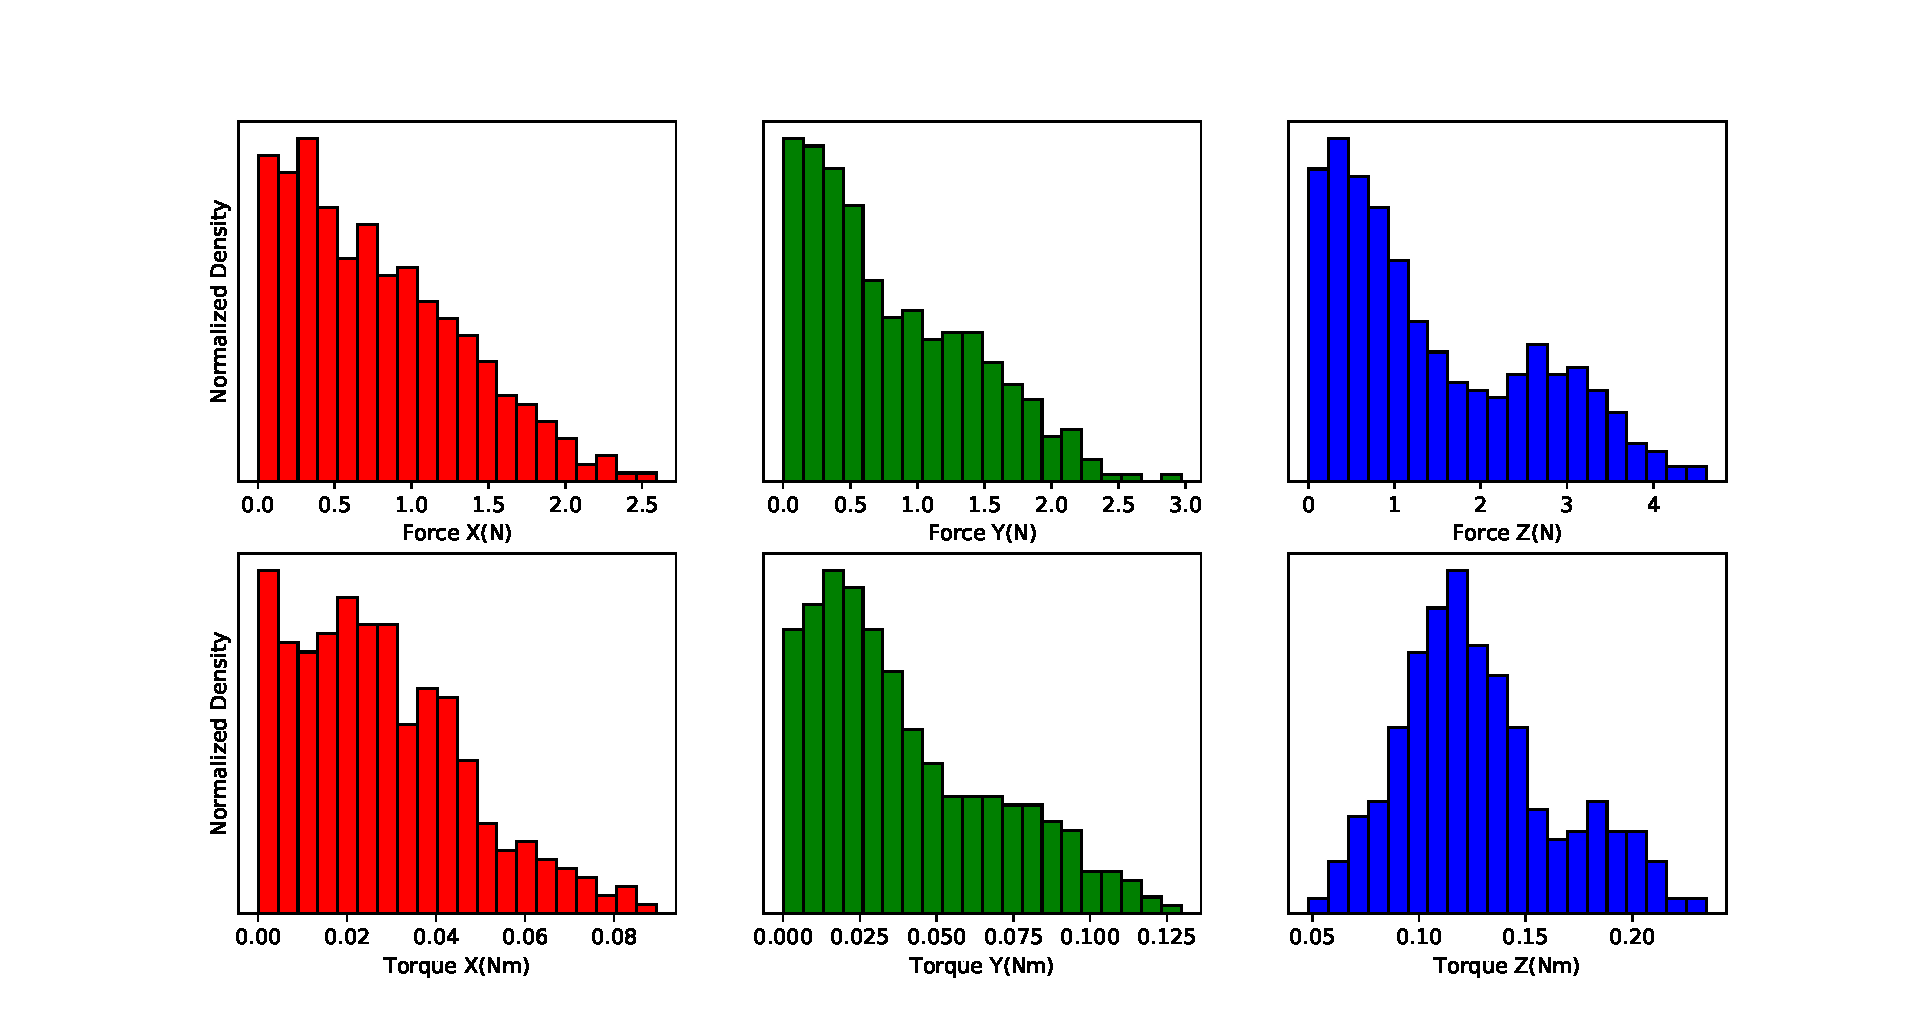
\includegraphics[width=\linewidth]{figs/chp3/ft_sensor_theory_hist.pdf}
    \caption{Visualization of the difference of the 2 things}
    \label{fig:ft_sensor_theory_hist}
\end{figure}

\par There is still some difference


\subsection{Correction of the FT Model based on Observations}

\par so aqui é que se fala das 57 posições e mais nao sei que

\begin{figure}[h]
    \centering
    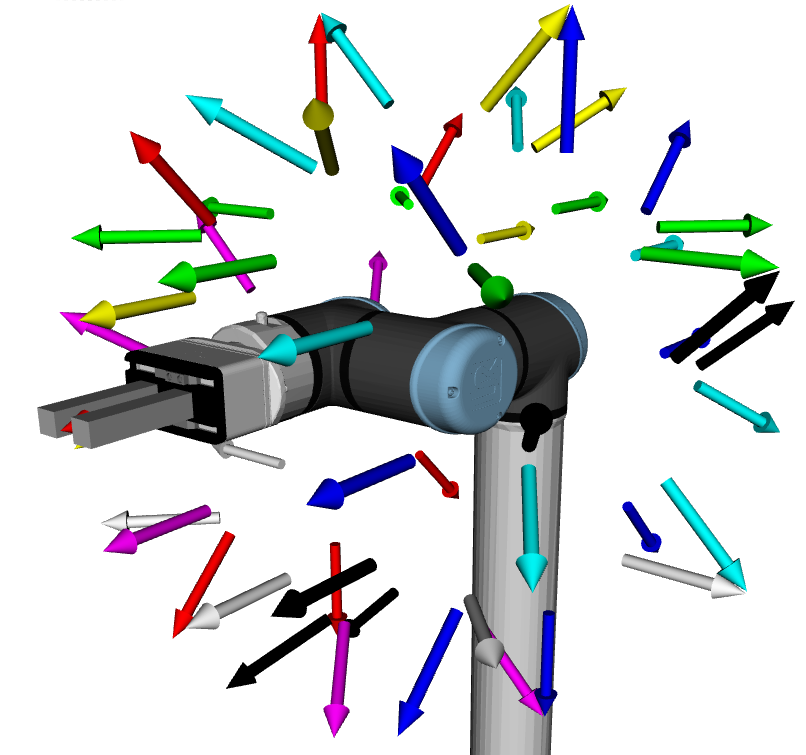
\includegraphics[width=0.35\linewidth]{figs/chp3/globe_57.png}
    \caption{Visualization of the 57 poses in which the tests were performed}
    \label{fig:57_poses}
\end{figure}

\par in each position a regular test was made and the result saved. then an optimization function was performed for each of them 

\par after inputing in the theoreticl model the results from the optimization function, the results obtained are as follow

% correr a função de otimização

\begin{figure}[h]
    \centering
    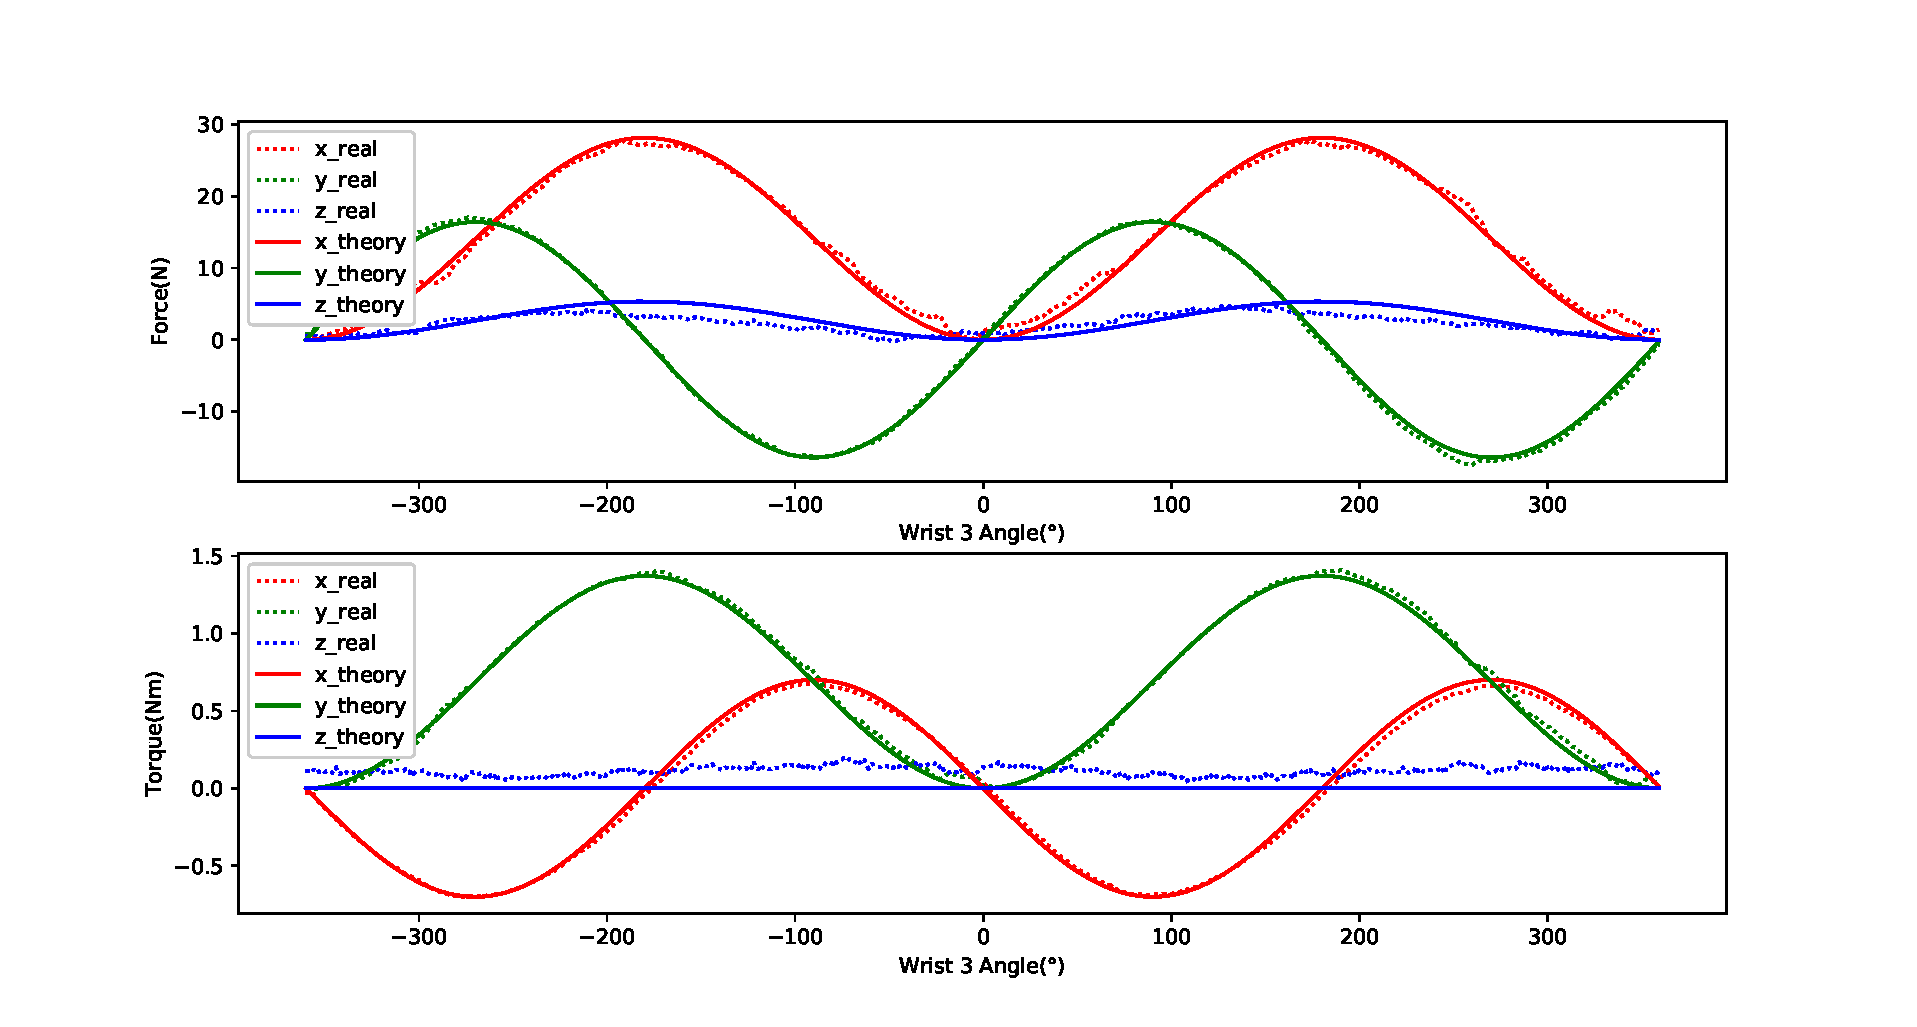
\includegraphics[width=\linewidth]{figs/chp3/ft_sensor_theory_adjust.pdf}
    \caption{Visualization of generation of theoretical torque values adjusted}
    \label{fig:ft_sensor_theory_adjust}
\end{figure}

\begin{figure}[h]
    \centering
    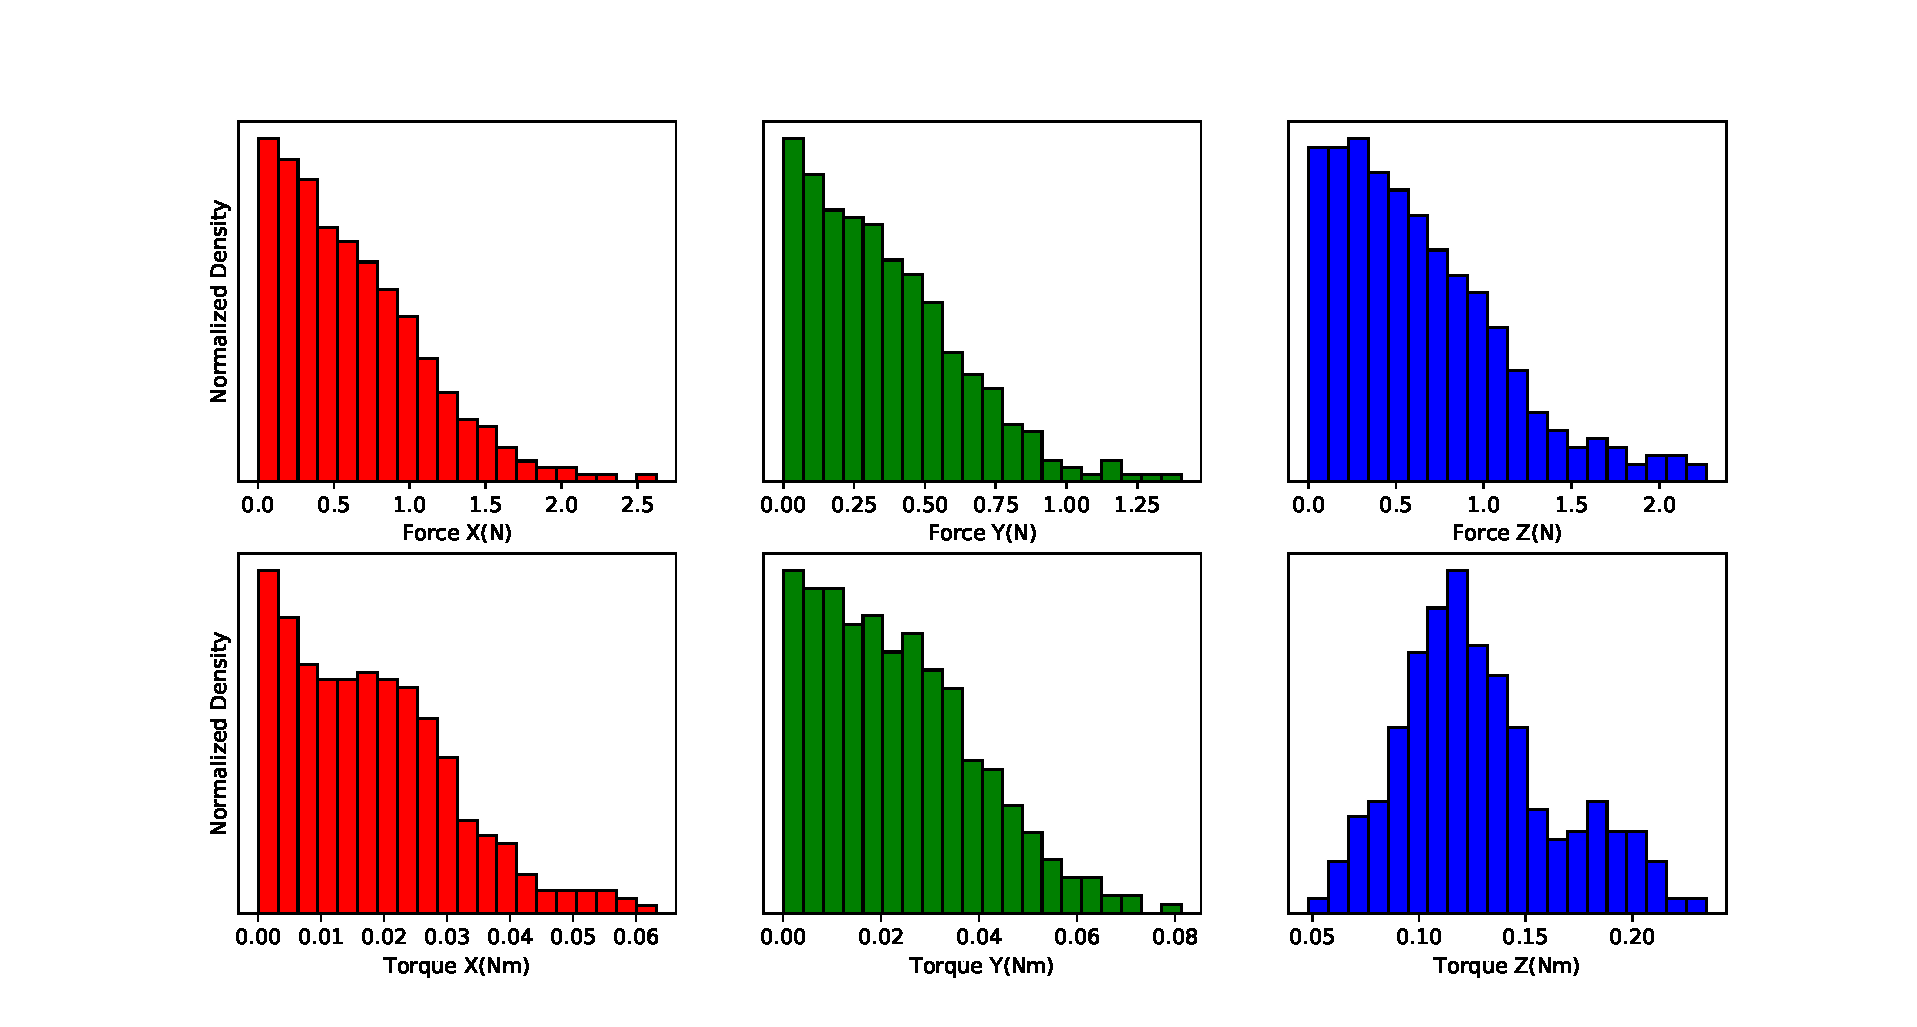
\includegraphics[width=\linewidth]{figs/chp3/ft_sensor_theory_adjust_hist.pdf}
    \caption{Visualization of the difference of the 2 things adjusted}
    \label{fig:ft_sensor_theory_adjust_hist}
\end{figure}

